\documentclass[aspectratio=169]{beamer}

\usepackage[utf8]{inputenc}

\usepackage{standalone}
\usepackage{caption}
\usepackage{amssymb, amsmath, amsthm, amsfonts}

\usepackage{tikz}
\usepackage{pgfplots}
\usetikzlibrary{shapes.geometric, arrows}
\usetikzlibrary{backgrounds}
\tikzstyle{node} = [rectangle]

\usepackage{float}

\newcommand{\comment}[1]{}

\usetheme{Dresden}
\usepackage[orientation=landscape,size=custom,width=16,height=9,scale=0.5,debug]{beamerposter}
\usepackage{animate}
\usepackage{url}

\title{N-body memory layout exploration}
\author{Oliver Geisel \& Lisa Hentschke}
\date{\today}


\begin{document}

\begin{frame}
	\titlepage
\end{frame}

\begin{frame}
	\frametitle{Structure}
	\tableofcontents
\end{frame}

\section{The task} 
\begin{frame}
	\frametitle{The n-body simulation}
	\begin{columns}
	\begin{column}{0.55\textwidth}
		\begin{itemize}
			\item simulate the interaction of \(n\) particles
			\item each particle has
			\begin{itemize}
				\smallskip
				\item position x
				\item position y
				\item position z
				\smallskip
				\item velocity x
				\item velocity y
				\item velocity z
				\smallskip
				\item mass
			\end{itemize}
		\end{itemize}
	\end{column}
	
	\begin{column}{0.45\textwidth}
		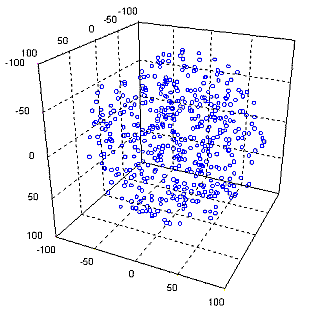
\includegraphics[scale=0.65]{resources/nbody.png}
		\tiny \url{http://astro.dur.ac.uk/~nm/pubhtml/nbody/nbody.html}
	\end{column}
	
	\end{columns}
	
\end{frame}

\begin{frame}
	\frametitle{Recap: AoS vs SoA}
	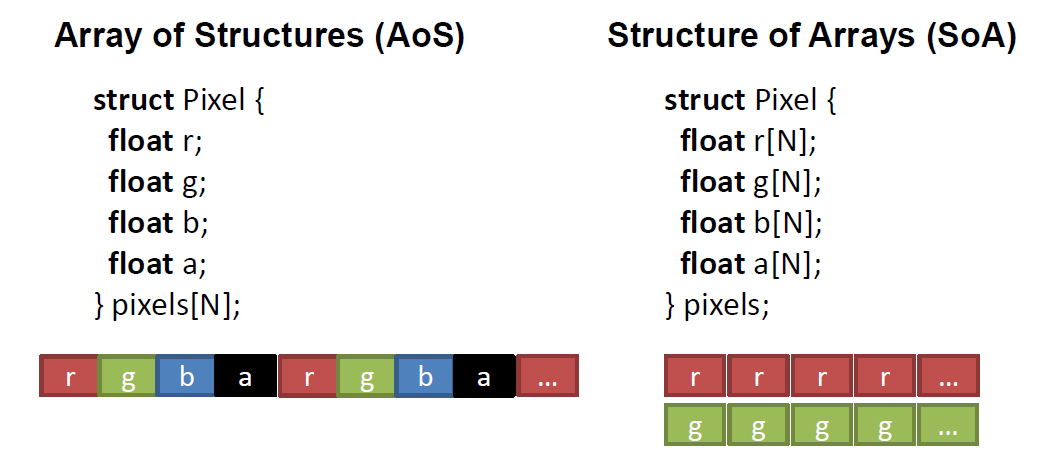
\includegraphics[scale=0.45]{resources/aos-vs-soa.png}
	
	\small from the slides 04-GPU-Memory
\end{frame}

\section{Solution Strategies}
\begin{frame}
	\frametitle{Solution Strategies}
	\begin{itemize}
		\item rewrite CPP-code in CUDA: implement AoS, SoA and AoSoA memory layouts
		\item implemented \underline{shared memory} variants
		\item for SoA: implemented two sub-variants: B and T
			\begin{itemize}
				\item B: compute one particle per block
				\item T: compute one particle per thread
			\end{itemize}
		\item We tested on several devices
	\end{itemize}
\end{frame}

\begin{frame}
	\frametitle{Example on K80}
	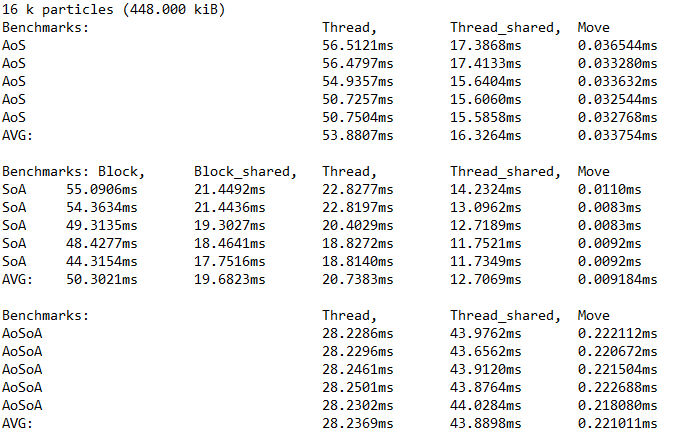
\includegraphics[scale=0.5]{resources/data-example.png}
\end{frame}


\section{Results}
\begin{frame}
	\frametitle{Used Profilers}
	\begin{columns}
	\begin{column}{0.3\textwidth}
		\begin{itemize}
			\small \item nvprof on Taurus
		\end{itemize}
	\end{column}
	
	\begin{column}{0.5\textwidth}
		\begin{itemize}
			\small \item Nvidia Visual Profiler version 11.2
		\end{itemize}
	\end{column}
	\end{columns}
	\medskip
	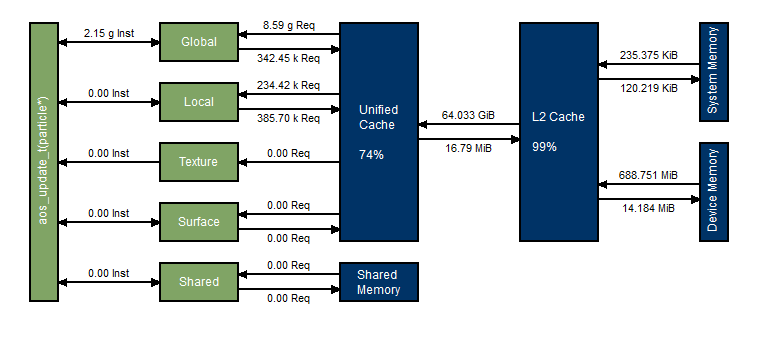
\includegraphics[scale=0.50]{resources/128-1070-aos-update-t.png}
	
	\smallskip
	\small tested on 1070; version 128k paricles on mem layout AoS; subversion T
\end{frame}

\begin{frame}
	\frametitle{Used Profilers}
	\begin{columns}
	\begin{column}{0.3\textwidth}
		\begin{itemize}
			\small \item nvprof on Taurus
		\end{itemize}
	\end{column}
	
	\begin{column}{0.5\textwidth}
		\begin{itemize}
			\small \item Nvidia Visual Profiler version 11.2
		\end{itemize}
	\end{column}
	\end{columns}
	\smallskip
	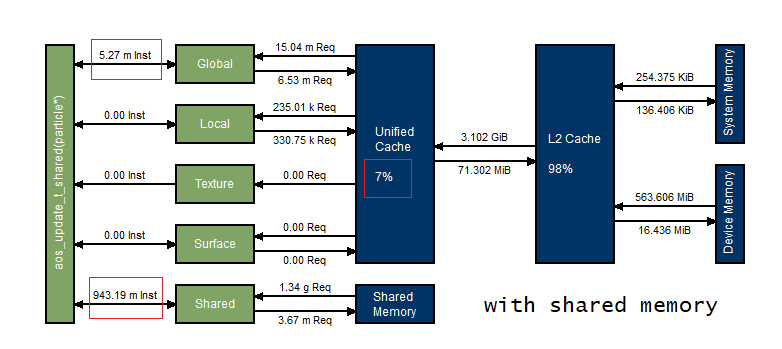
\includegraphics[scale=0.50]{resources/128-1070-aos-update-t-shared.png}
	
	\smallskip
	\small tested on 1070; version 128k paricles on mem layout AoS; subversion T
\end{frame}

\begin{frame}
	\frametitle{Compare the memory structures}
	We tested on K80 (Taurus), v100 (Taurus), 1070 (private, driver version 461.09), and RTX 2080 (private, driver version 641.40) respectively
	
	\medskip
	Memory Layout:
	\begin{itemize}
		\item K80 - GDDR 5 with SDRAM
		\item v100 - HBM 2
		\item 1070 - GDDR 5
		\item RTX 2080 - GDDR 6
	\end{itemize}
\end{frame}

\begin{frame}
	\frametitle{Compare the memory structures - on K80}
	\begin{columns}
	\begin{column}{0.25\textwidth}
	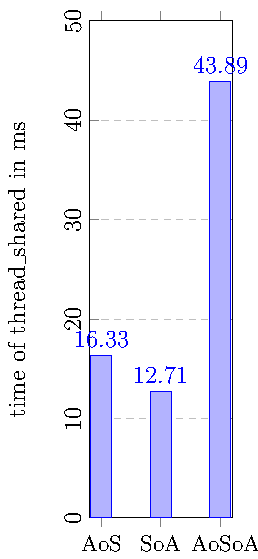
\includegraphics[scale=0.55]{figures/fig1.pdf}
	\small 16K
	\end{column}
	%===========
	\begin{column}{0.25\textwidth}
	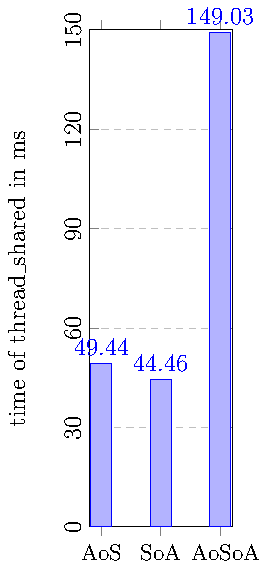
\includegraphics[scale=0.55]{figures/fig2.pdf}
	\small 32K
	\end{column}
	%===========
	\begin{column}{0.25\textwidth}
	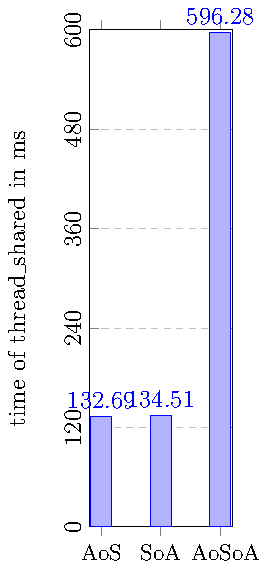
\includegraphics[scale=0.55]{figures/fig3.pdf}
	\small 64K
	\end{column}
	%===========
	\begin{column}{0.25\textwidth}
	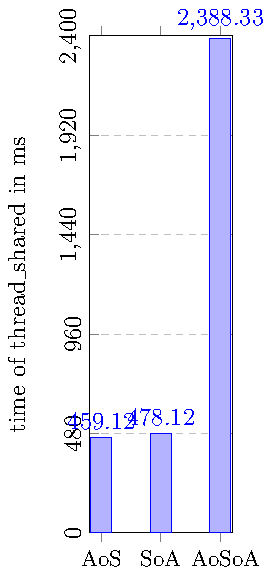
\includegraphics[scale=0.55]{figures/fig4.pdf}
	\small 128K
	\end{column}	
	\end{columns}
	
\end{frame}


\begin{frame}
	\frametitle{Compare the memory structures - on v100}
	\begin{columns}
	\begin{column}{0.25\textwidth}
	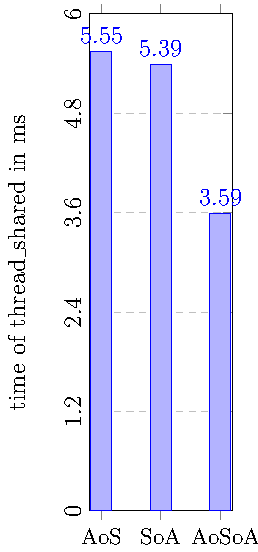
\includegraphics[scale=0.55]{figures/fig10.pdf}
	\small 16K
	\end{column}
	%===========
	\begin{column}{0.25\textwidth}
	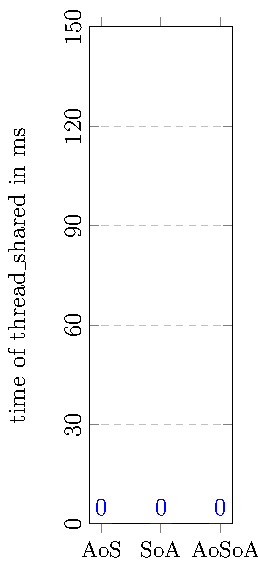
\includegraphics[scale=0.55]{figures/fig20.pdf}
	\small 32K
	\end{column}
	%===========
	\begin{column}{0.25\textwidth}
	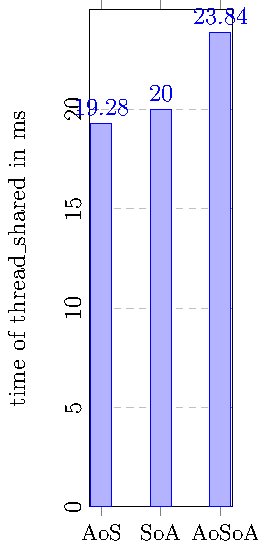
\includegraphics[scale=0.55]{figures/fig30.pdf}
	\small 64K
	\end{column}
	%===========
	\begin{column}{0.25\textwidth}
	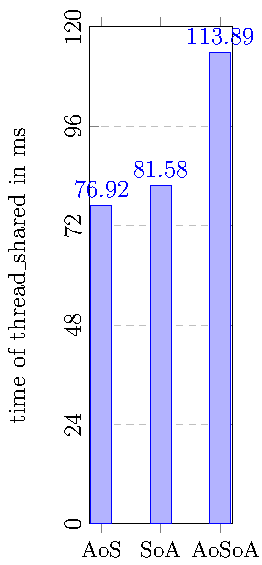
\includegraphics[scale=0.55]{figures/fig40.pdf}
	\small 128K
	\end{column}	
	\end{columns}
	
\end{frame}


\begin{frame}
	\frametitle{Compare the memory structures - on 1070}
	\begin{columns}
	\begin{column}{0.25\textwidth}
	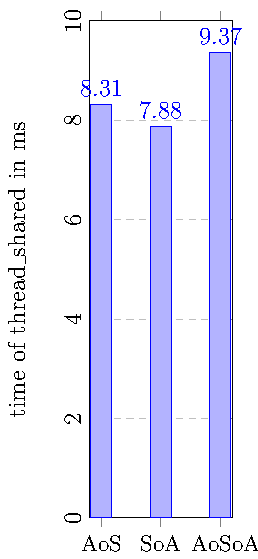
\includegraphics[scale=0.55]{figures/fig100.pdf}
	\small 16K
	\end{column}
	%===========
	\begin{column}{0.25\textwidth}
	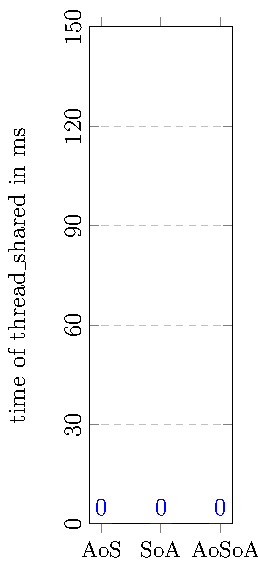
\includegraphics[scale=0.55]{figures/fig200.pdf}
	\small 32K
	\end{column}
	%===========
	\begin{column}{0.25\textwidth}
	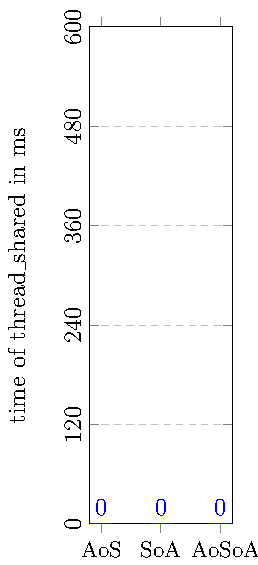
\includegraphics[scale=0.55]{figures/fig300.pdf}
	\small 64K
	\end{column}
	%===========
	\begin{column}{0.25\textwidth}
	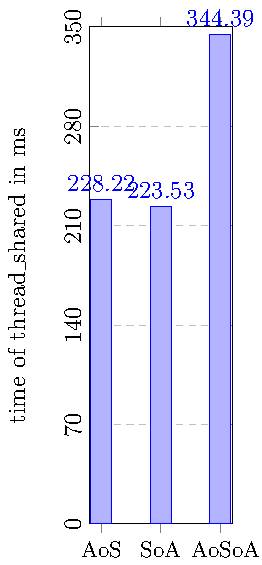
\includegraphics[scale=0.55]{figures/fig400.pdf}
	\small 128K
	\end{column}	
	\end{columns}
	
\end{frame}


\begin{frame}
	\frametitle{Compare the memory structures - on RTX 2080}
	\begin{columns}
	\begin{column}{0.25\textwidth}
	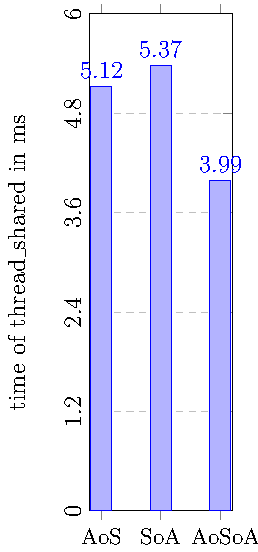
\includegraphics[scale=0.55]{figures/fig1000.pdf}
	\small 16K
	\end{column}
	%===========
	\begin{column}{0.25\textwidth}
	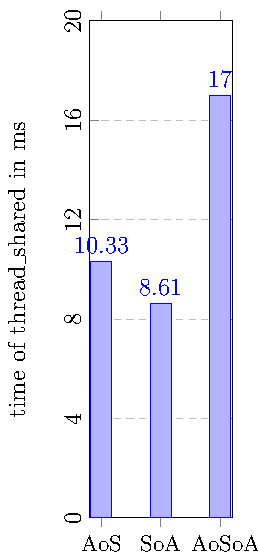
\includegraphics[scale=0.55]{figures/fig2000.pdf}
	\small 32K
	\end{column}
	%===========
	\begin{column}{0.25\textwidth}
	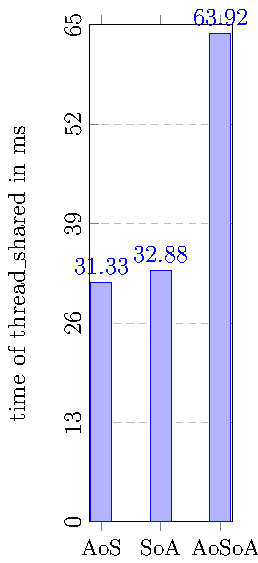
\includegraphics[scale=0.55]{figures/fig3000.pdf}
	\small 64K
	\end{column}
	%===========
	\begin{column}{0.25\textwidth}
	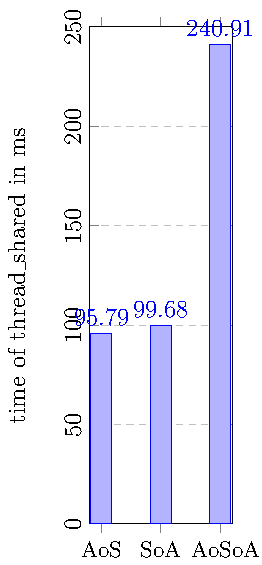
\includegraphics[scale=0.55]{figures/fig4000.pdf}
	\small 128K
	\end{column}	
	\end{columns}
	
\end{frame}

\begin{frame}
	\frametitle{Conclusion}
	\begin{itemize}
		\item AoSoA can be optimized, but ...
		\item AoS or SoA heavily depends on architecture \(\rightarrow\) just take the easier implementation
	\end{itemize}
\end{frame}


\section{Explanation}
\begin{frame}
	\frametitle{Performance of AoSoA on 16K}
	\begin{itemize}
		\item has nothing to do with the mem layout
		\item SMs aren't fully occupied
		\item we configured 32 threads per block
	\end{itemize}
\end{frame}

\begin{frame}
	\frametitle{AoS vs SoA}
	\begin{itemize}
		\item performance AoS vs SoA are somewhat equally
		\item contrary to facts from the lecture \(\rightarrow\) WHY?
		\item K80, v100, and RTX 2080 have configurable L1 chaches (we chose 32KiB)
		\item also read-only data cache for K80 (48KiB), for 1070 (no RODC) \(\rightarrow\) AoS behaves differently
		\item that could be the reason why AoS can be better than SoA (bigger chache)
		\item guess: at bigger  \(n\) AoS can't catch up? but ...
	\end{itemize}
\end{frame}

\begin{frame}
	\frametitle{On v100 with 2 million particles}
	\begin{columns}
	\begin{column}{0.25\textwidth}
	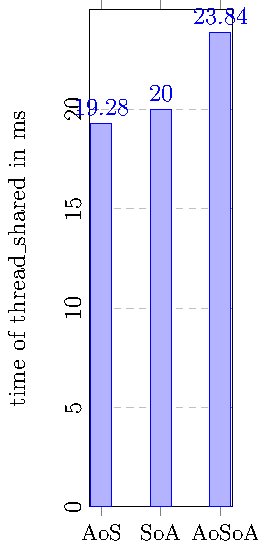
\includegraphics[scale=0.55]{figures/fig30.pdf}
	\small 64K
	\end{column}
	%===========
	\begin{column}{0.25\textwidth}
	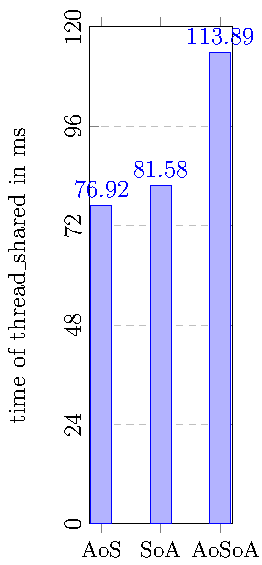
\includegraphics[scale=0.55]{figures/fig40.pdf}
	\small 128K
	\end{column}
	%===========
	\begin{column}{0.25\textwidth}
	\large ...
	\end{column}	
	%===========
	\begin{column}{0.25\textwidth}
	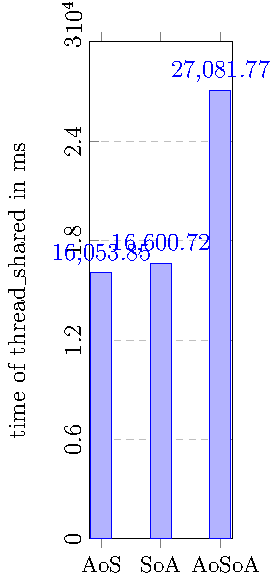
\includegraphics[scale=0.55]{figures/fig50.pdf}
	\small 2M
	\end{column}	
	\end{columns}
	
\end{frame}

\begin{frame}
	\frametitle{The Explanation?}
	\begin{itemize}
		\item we don't really know
		\item cache hierarchy is dynamic and complex, e.g.
	\end{itemize}
	\bigskip
	
		\begin{tabular}{ |r|| c | c c| }
			\hline
			K80 & 48 RODC & dyn. 16-48 L1 & (it's 32 in our case)\\
			\hline
			V100 & 128 UDC & rest L1 & (it's 96 in our case)\\
			\hline
			RTX 2080 & 96 UDC & rest L1 & (it's 64 in our case)\\
			\hline
			1070 & -- RODC & 48 L1 &\\
			\hline
		\end{tabular}
		
	\small *values are given in KiB
	\smallskip
	
	\small RODC ... read-only data cache
	
	\small UDC ... unified memory cache
\end{frame}


\comment{
\begin{frame}
	\frametitle{General Performance}
	\begin{itemize}
		\item at small \(n <\) 1K CPU is usually faster
	\end{itemize}
\end{frame}
} %end comment


\section{Further Approaches}
\begin{frame}
	\frametitle{What else could we try?}
	\begin{itemize}
		\item use texture memory (indirectly we already do that)
		\begin{itemize}
			\item \(\rightarrow\) mass never changes
		\end{itemize}
		\item use surface memory? tensor cores?
		\item change computation (not part of the task)
		\item optimize AoSoA (not sure if it will be better compared to SoA)
	\end{itemize}
\end{frame}

\section{Validation}
\begin{frame}
	\frametitle{Validation}
	Two ways:
	\begin{itemize}
		\item  \textbf{visualize} a 3-body problem with our code, see if it's right
		\item  \textbf{compare} with reference computation (use reference values)
	\end{itemize}
\end{frame}

\end{document}